\documentclass{article}
\usepackage[italian]{babel}
\usepackage[tmargin=2cm,rmargin=1.5in,lmargin=1.5in,margin=0.85in,bmargin=2cm,footskip=.2in]{geometry}
\usepackage{siunitx}
\sisetup{separate-uncertainty=true, per-mode=fraction, parse-numbers=true}
\usepackage{caption}
\usepackage[T1]{fontenc}
\usepackage{bookmark}
\usepackage{graphicx}
\usepackage{multicol}
\usepackage{booktabs}
\usepackage{amsmath,amsfonts,amsthm,amssymb,mathtools}
\hypersetup{
	pdftitle={Appunti Tomadin},
	colorlinks=true, linkcolor=doc!90,
	bookmarksnumbered=true,
	bookmarksopen=true
}
\usepackage{blindtext}
\usepackage{wrapfig}
\usepackage{listings}
\usepackage{xcolor}
\usepackage{float}
\usepackage{tikz}
\usepackage{multirow}
\usepackage{biblatex}
\definecolor{codegreen}{rgb}{0,0.6,0}
\definecolor{codegray}{rgb}{0.5,0.5,0.5}
\definecolor{codepurple}{rgb}{0.58,0,0.82}
\definecolor{backcolour}{rgb}{0.95,0.95,0.92}
\definecolor{doc}{rgb}{0,0,0}
\lstdefinestyle{code}{
    backgroundcolor=\color{backcolour},   
    commentstyle=\color{codegreen},
    keywordstyle=\color{magenta},
    numberstyle=\tiny\color{codegray},
    stringstyle=\color{codepurple},
    basicstyle=\ttfamily\footnotesize,
    breakatwhitespace=false,         
    breaklines=true,                 
    captionpos=b,                    
    keepspaces=true,                                     
    showspaces=false,                
    showstringspaces=false,
    showtabs=false,                  
    tabsize=2,
    inputencoding=ansinew,
    extendedchars=true,
    numbers=left,                    
    numbersep=5pt
}

\lstset{style=code}
\usepackage[varbb]{newpxmath}
\usepackage{circuitikz}
\title{Relazione sui rimbalzi di una pallina}
\author{Aiello Giosuè, Fenili Domenico, Sermi Francesco}
\date{\today}

\begin{document}
\maketitle
\pagebreak
\tableofcontents
\pagebreak
\section{Titolo}
Determinare la validità del modello teorico scelto per una pallina che cade rimbalzando su una superficie rigida
\section{Premesse teoriche}
Nel modello più semplice ipotizzabile per una pallina che cade rimbalzando, possiamo supporre che questa perda una frazione $\gamma$ indipendentemente dalla velocità posseduta prima della caduta. Se lasciamo cadere quindi una pallina da un'altezza nota $h_0$ con velocità iniziale nulla:
\begin{equation}
	h_n = h_0 \gamma ^n
\end{equation}
dove $n$ rappresenta il numero di rimbalzi. In questo modello è facilmente dimostrabile che l'altezza massima raggiungibile può essere determinata partendo dai tempi di rimbalzo con la seguente formula, sebbene non tenga conto di effetti come la resistenza dell'aria:
\begin{equation}
	h_n = \frac{1}{8} g (t_n - t_{n-1})^2
\end{equation}
\section{Strumenti e materiali}
Per effettuare questa esperienza abbiamo utilizzato i seguenti materiali:
\begin{itemize}
	\item una pallina da tennis, abbastanza elastica;
	\item un metro a nastro
\end{itemize}
Per quanto riguarda gli strumenti abbiamo invece utilizzato:
\begin{itemize}
	\item \textbf{Audacity}, software per l'elaborazione dei file audio;
	\item uno smartphone, per registrare dei file audio;
\end{itemize}
\section{Descrizione sulle misure}
Prima di procedere con le misure sono state effettuate facendo una serie di registrazioni di prova per verificare quale fosse l'altezza ottimale per effettuare il maggior numero di misurazioni. \\ La pallina, in base al materiale di cui è fatta, perderà una maggiore o una minore frazione di energia cinetica ad ogni urto, urtando più o meno volte contro il pavimento, pertanto dovevamo individuare l'altezza $h_0$ da cui era possibile ottenere un buon numero di urti. Oltre a ciò queste prove si sono rivelate utili per individuare la posizione dello smartphone migliore per misurare in maniera più efficace la pressione sonora esercitata dagli urti della pallina contro il pavimento (un accorgimento che si rivelerà molto utile nel momento in cui verranno fatte le analisi sul campione audio registrato). \\ \textbf{Considerazioni}: nel nostro setup sperimentale, fino ad ora le uniche fonti di errori possono derivare dalla possibilità pallina urti contro altri oggetti presenti nelle vicinanze e siano presenti dei rumori che possono invalidare la registrazione audio effettuata con lo smartphone. Per ovviare a questo problema abbiamo deciso di lavorare in un ambiente spazioso e il più silenzioso possibile. 

\begin{wrapfigure}{l}{0.5\textwidth}
	\vspace{-0.5cm}
	\begin{lstlisting}[language=Python]
	import wave
	import numpy as np
	from matplotlib import pyplot as plt
	stream = wave.open("./Audio.wav")
	signal = np.frombuffer(stream.readframes(stream.getnframes()), dtype=np.int16)
	t = np.arange(len(signal)) / stream.getframerate()
	plt.figure("Rimbalzi pallina")
	plt.plot(t, signal)
	plt.xlabel("Tempo [s]")
	plt.savefig("Grafico_rimbalzo.pdf")
	plt.show()
	\end{lstlisting}
\end{wrapfigure}

\noindent \\ Successivamente abbiamo effettuato le misure. Dopo aver raccolto il campione audio, siamo passati ad analizzarlo con la libreria \emph{matplotlib}. Non disponendo di un'applicazione per la registrazione dei suoni in grado di registrare in formato \emph{.wave} abbiamo utilizzato il software \textbf{Audacity} per convertire il file in un formato in grado di essere letto dalla libreria. Il codice usato per rappresentare il campione audio è riportato qua di lato. \\ \\
\newpage

\begin{wrapfigure}{r}{0.5\textwidth}
	\centering
	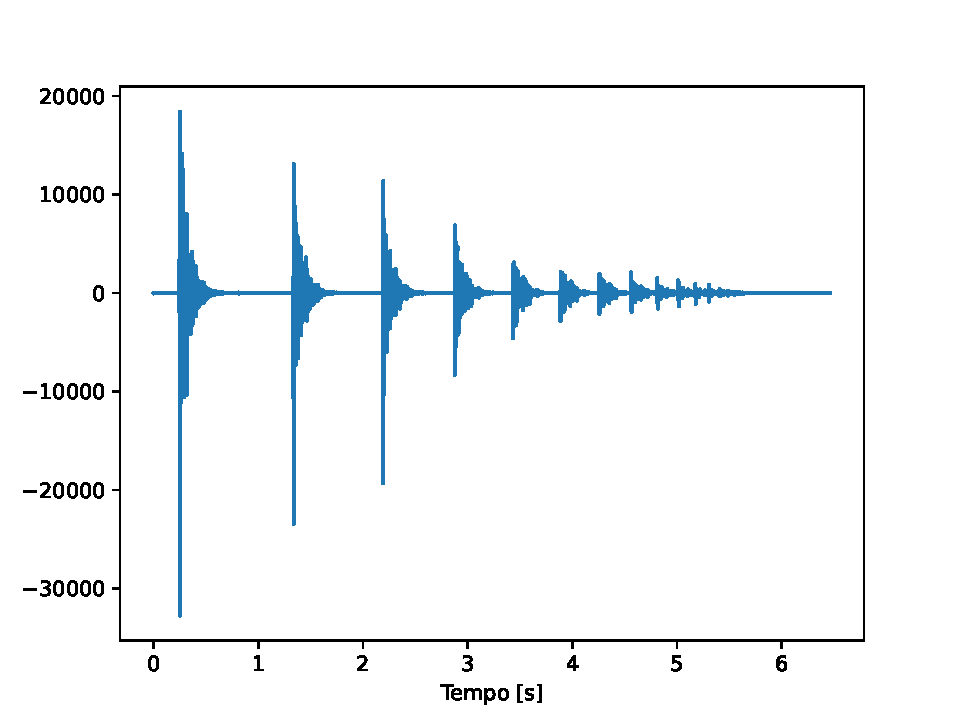
\includegraphics[width=0.4\textwidth, scale=0.25]{Grafico_rimbalzo.pdf}
	\caption{Immagine audio del campione audio misurato dal telefono: ogni rimbalzo della pallina è caratterizzato da un attacco più lungo ed una coda relativamente più lunga e già si intuisce il problema di individuare l'intervallo in cui è avvenuto l'urto}
	\label{fig:audio}
\end{wrapfigure}

La determinazione degli istanti in cui è avvenuto il rimbalzo è la fase più delicata della raccolta dati di questa esperienza e quello più soggetta agli errori accidentali e sistematici. Come si può vedere dalla \ref{fig:audio} qua di lato, infatti, non è possibile individuare in maniera precisa l'\emph{esatto} istante temporale in cui è avvenuto il rimbalzo a causa della natura impulsiva delle forze che hanno agito sulla pallina. \\
Siccome ogni rimbalzo è caratterizzato da un picco, abbiamo considerato l'istante del rimbalzo come il valore medio dell'intervallo di tempo che va dall'istante in cui la pressione sonora è massima all'istante di tempo successivo con un nuovo picco massimo relativo.

\section{Analisi dei dati}

Per questa analisi abbiamo utilizzato il metodo del parametro libero del fit rispetto al valore $h_0$. Abbiamo realizzato con il linguaggio di programmazione Python e la funzione \emph{curve\_fit} della libreria \emph{scipy} un grafico delle altezze $h_n$ in funzione dell'indice $n$ che rappresenta l'$n$-esimo rimbalzo della pallina. \\
Siccome il modello teorico che avevamo ipotizzato era della forma:
$$
	h_n = h_0 \gamma^n
$$
dovrebbe risultare che i nostri dati si dispongono come un esponenziale e quindi dovrebbero apparire come una retta in scala semilogaritmica. Inoltre,  tenendo $h_0$ come parametro libero, possiamo confrontare il valore stimato dal fit con quello reale per valutare di quanto si discosta dalla realtà il modello teorico. \\
Per quanto riguarda la determinazione degli errori, abbiamo considerato 	

\section{Appendice}
\subsection{Codice Python utilizzato}
Per la realizzazione di questa esperienza, abbiamo utilizzato il seguente codice \emph{Python}
\begin{lstlisting}[language=Python]

\end{lstlisting}
\end{document}